\documentclass[12pt,a4paper]{article}
\usepackage{cmap} % Makes the PDF copiable. See http://tex.stackexchange.com/a/64198/25761
\usepackage[T1]{fontenc}
\usepackage[brazil]{babel}
\usepackage[utf8]{inputenc}
\usepackage{amsmath}
\usepackage{amsfonts}
\usepackage{amssymb}
\usepackage{amsthm}
\usepackage[usenames,svgnames,dvipsnames]{xcolor}
\usepackage{hyperref}
\usepackage{multicol}
\usepackage{graphicx}
\usepackage[margin=2cm]{geometry}

\hypersetup{
    colorlinks = true,
    allcolors = {blue}
}

% TODO: Consider using exsheets
% http://linorg.usp.br/CTAN/macros/latex/contrib/exsheets/exsheets_en.pdf
%
% http://ctan.org/tex-archive/macros/latex/contrib/exercise/
% Options: answerdelayed,lastexercise,noanswer
\usepackage[answerdelayed,lastexercise]{exercise}

\addto\captionsbrazil{%
\def\listexercisename{Lista de exerc\'icios}%
\def\ExerciseName{Exerc\'icio}%
\def\AnswerName{Solu\c{c}\~ao do exerc\'icio}%
\def\ExerciseListName{Ex.}%
\def\AnswerListName{Solu\c{c}\~ao}%
\def\ExePartName{Parte}%
\def\ArticleOf{de\ }%
}

\renewcommand{\ExerciseHeaderTitle}{(\ExerciseTitle)\ }
\renewcommand{\ExerciseListHeader}{%\ExerciseHeaderDifficulty%
\textbf{%\ExerciseListName\
\ExerciseHeaderNB.\ %
%\ --- \
\ExerciseHeaderTitle}%
%\ExerciseHeaderOrigin
\ignorespaces}
\renewcommand{\AnswerListHeader}{\textbf{\ExerciseHeaderNB.\ (\AnswerListName)\ }}

\newtheorem*{note}{Observação}
\newcommand{\fixme}{{\color{red}(...)}}
\newcommand*\diff{\mathop{}\!\mathrm{d}}
\newcommand*\sen{\operatorname{sen}}
\newcommand*\tg{\operatorname{tg}}
\newcommand*\cotg{\operatorname{cotg}}
\newcommand*\cosec{\operatorname{cossec}}
\newcommand*\cotgh{\operatorname{cotgh}}
\newcommand*\arcsen{\operatorname{arcsen}}
\newcommand*\arctg{\operatorname{arctg}}
\newcommand*\abs[1]{\left|#1\right|}
\newcommand*\R{\mathbb{R}}
\newcommand*\op[1]{\overset{#1}{\rightarrow}}

\renewcommand{\theenumi}{\alph{enumi}}
\renewcommand\labelenumi{(\theenumi) }

\newcommand*\tipo{Prova II}
\newcommand*\turma{CIV241-02U}
\newcommand*\disciplina{CDI2002}
\newcommand*\eu{Helder G. G. de Lima}
\newcommand*\data{22/10/2024}

\author{\eu}
\title{\tipo - \disciplina}
\date{\data}

\begin{document}
\thispagestyle{empty}
\newgeometry{margin=2cm,bottom=0.5cm}
\begin{center}

\includegraphics[width=9.0cm]{marca} \\
\textbf{\tipo\ (\disciplina / \turma)} \\
Prof. \eu\footnote{
Este é um material de acesso livre distribuído sob os termos da licença \href{https://creativecommons.org/licenses/by-sa/4.0/deed.pt_BR}{Creative Commons BY-SA 4.0}}
\end{center}

\noindent Nome do(a) aluno(a): \underline{\hspace{9,7cm}} Data: \underline{\data}

\begin{center}\fbox{
\begin{minipage}{14cm}

{\footnotesize
\begin{itemize}
\renewcommand{\theenumi}{\Roman{enumi}}
\item Identifique-se em todas as folhas.
\item Mantenha o celular e os demais equipamentos eletrônicos desligados durante a prova.
\item Justifique cada resposta com cálculos ou argumentos baseados na teoria estudada.
\item Resolva $4$ das $5$ questões (deixe claro que questão não deverá ser corrigida).
\end{itemize}
}

\end{minipage}
}
\end{center}

\begin{ExerciseList}
\Exercise[title={2,5}] Calcule o volume do sólido gerado pela rotação, em torno do eixo $x$, da região delimitada pelo gráfico da função $f(x) = \tan(x)$, e pelas retas verticais $x = 0$ e $x = \frac{\pi}{4}$.
\Answer O volume do sólido formado pela revolução de \( y = \tan(x) \) de \( x = 0 \) a \( x = \frac{\pi}{4} \) em torno do eixo $x$ é dado pela fórmula:
\[
V = \int_0^{\frac{\pi}{4}} \pi [\tan(x)]^2 \diff{x}.
\]

Como \( [\tan(x)]^2 = \sec^2(x) - 1 \), obtemos:

\begin{align*}
    V
    &
    = \pi \int_0^{\frac{\pi}{4}} [\tan(x)]^2 \diff{x}
    = \pi \int_0^{\frac{\pi}{4}} (\sec^2(x) - 1) \diff{x}
    = \pi [ \tan(x) - x ] \bigg|_0^{\frac{\pi}{4}} \\
    &
    = \pi \left[ \left( \tan\left(\frac{\pi}{4}\right) - \frac{\pi}{4} \right) - \left( \tan(0) - 0 \right) \right]
    = \pi \left[ \left( 1 - \frac{\pi}{4} \right) - \left( 0 - 0 \right)\right]
    = \boxed{\pi - \frac{\pi^2}{4} \text{ u.v.}}.
\end{align*}

\begin{center}
    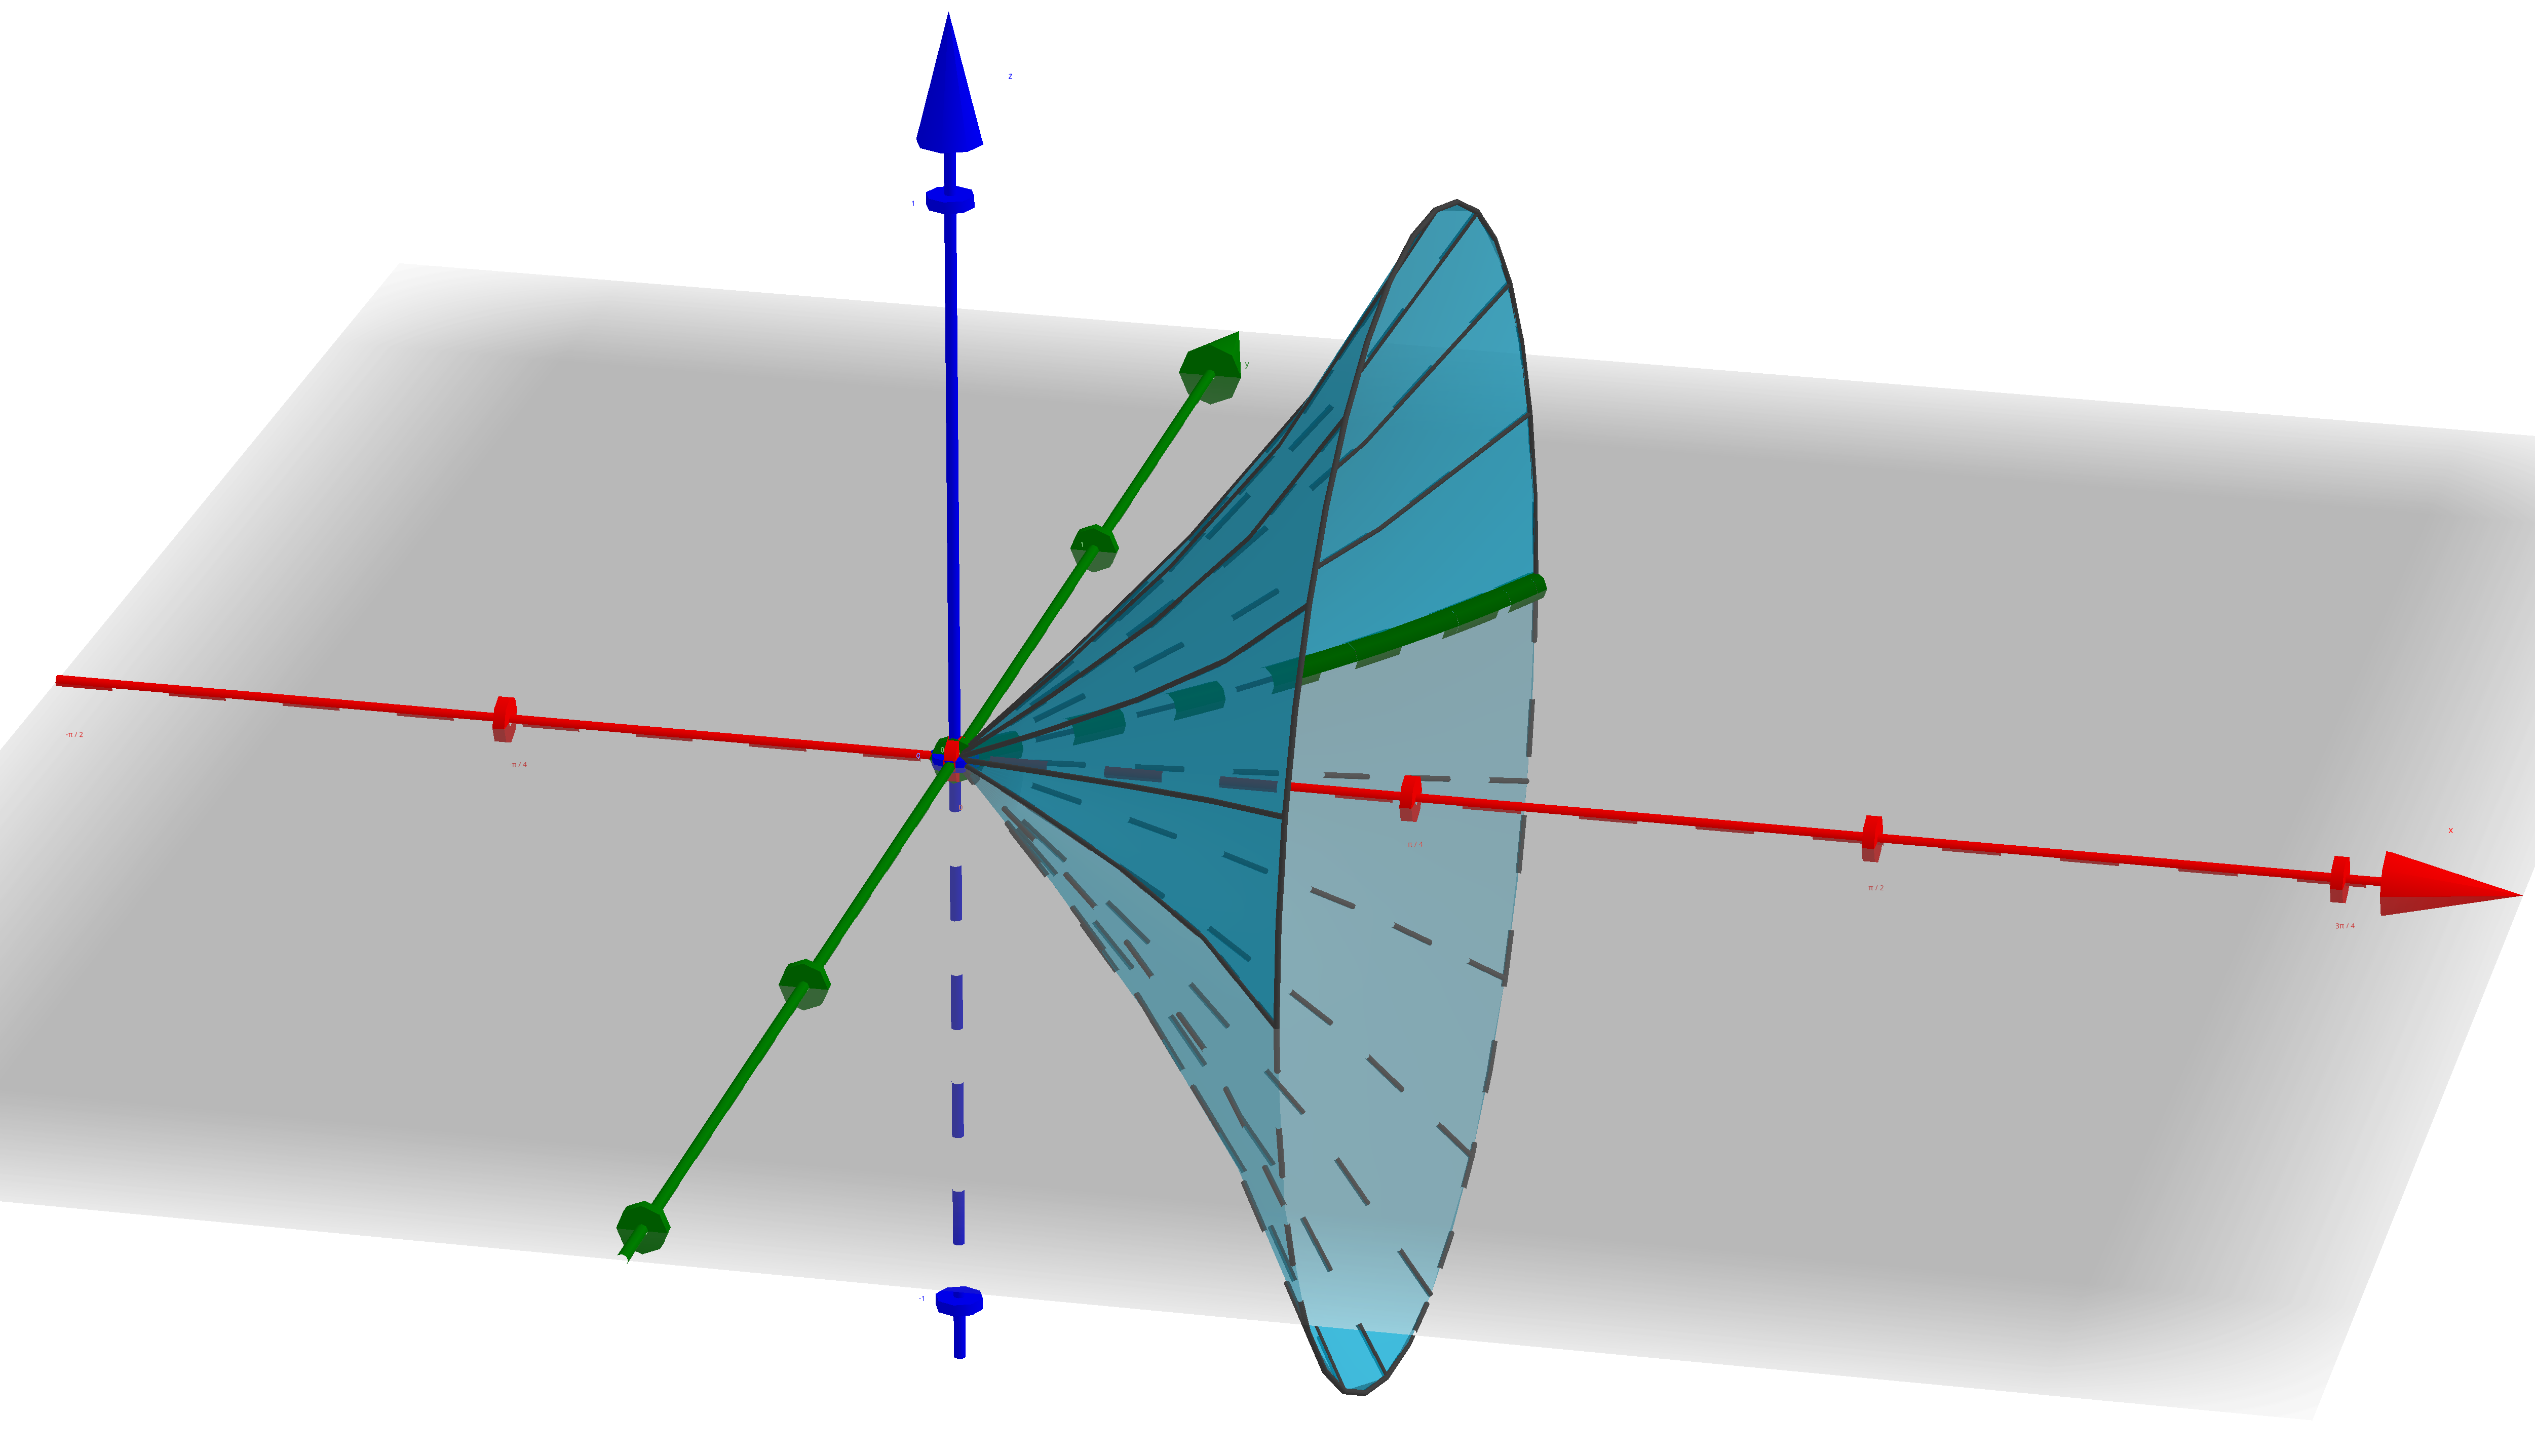
\includegraphics[height=4cm]{img/1-sólido-de-revolução.png}
\end{center}

\Exercise[title={2,5}] Determine se a série \(\sum_{n=1}^{\infty} \frac{2+9^n}{10^n + 2024}\) converge ou diverge.

\Answer Como a série não tem termos negativos, podemos utilizar o teste da comparação. Observe que

\[
\frac{2+9^n}{10^n + 2024}
\leq \frac{2+9^n}{10^n}
= \frac{2}{10^n} + \left(\frac{9}{10}\right)^n
= 2 \left(\frac{1}{10}\right)^n + \left(\frac{9}{10}\right)^n, \forall n \in \mathbb{N}^*.
\]

Como \(\frac{1}{10} < 1\) e \(\frac{9}{10} < 1\), as séries geométricas
\(\sum_{n=1}^{\infty} \frac{2}{10} \cdot \left(\frac{1}{10}\right)^{n-1}\)
e
\(\sum_{n=1}^{\infty} \frac{9}{10} \cdot \left(\frac{9}{10}\right)^{n-1}\)
são convergentes, e consequentemente a série
\(\sum_{n=1}^{\infty} \left(\frac{2}{10^n} + \left(\frac{9}{10}\right)^n\right)\)
também é convergente.

Portanto, pela comparação, a série original \(\boxed{\sum_{n=1}^{\infty} \frac{2+9^n}{10^n + 2024} \text{ é convergente}}\).

\textbf{Observações}:
\begin{itemize}
\item É preciso usar algum teste de convergência pois a série satisfaz a condição necessária para convergência:
\[
\lim_{n\to\infty} \frac{2+9^n}{10^n + 2024}
= \lim_{n\to\infty} \frac{9^n \ln(9)}{10^n \ln(10)}
= \frac{\ln(9)}{\ln(10)} \cdot \lim_{n\to\infty} \left(\frac{9}{10}\right)^n
= 0.
\]
\item O teste da comparação não nos permitiria tirar qualquer conclusão ao comparar $\frac{2+9^n}{10^n + 2024}$ diretamente com $\frac{9^n}{10^n}$ já que, embora \(\sum_{n=1}^{\infty} \left(\frac{9}{10}\right)^n\) seja convergente, temos $\frac{2+9^n}{10^n + 2024} > \frac{9^n}{10^n}$, para $n$ suficientemente grande (verifique!).
\item Para comparar $\frac{2+9^n}{10^n + 2024}$ diretamente com o termo geral de uma única série geométrica, uma opção seria observar que:

\[
\frac{2+9^n}{10^n + 2024}
\leq \frac{2+9^n}{10^n}
\leq \frac{2\cdot 9^n +9^n}{10^n}
= \frac{3\cdot 9^n}{10^n}
= 3 \cdot \left(\frac{9}{10}\right)^n, \forall n \in \mathbb{N}^*.
\]
\item O teste da razão também permite concluir que a série é convergente , pois
\[
L = \lim_{n \to \infty} \left|\frac{\frac{2+9^{n+1}}{10^{n+1} + 2024}}{\frac{2+9^n}{10^n + 2024}}\right| = \ldots = \frac{9}{10} < 1
\]
\end{itemize}


\Exercise[title={2,5}] Determine o raio e o intervalo de convergência da série de potências \(\sum_{n=1}^{\infty} \frac{(x-5)^n}{n^2}\).

\Answer Vamos usar o teste da razão, considerando $a_n = \frac{(x-5)^n}{n^2}$. Como
\[
    \left| \frac{a_{n+1}}{a_n} \right|
    = \left| \frac{\frac{(x-5)^{n+1}}{(n+1)^2}}{\frac{(x-5)^n}{n^2}} \right|
    = \left| \frac{(x-5)^{n+1}}{(n+1)^2} \cdot \frac{n^2}{(x-5)^n} \right|
    = \left| \frac{n^2}{(n+1)^2} \cdot (x-5) \right|
    = \frac{n^2}{(n+1)^2} \cdot \left| x-5 \right|,
\]
então
\begin{align*}
\lim_{n \to \infty} \left| \frac{a_{n+1}}{a_n} \right|
&
= \lim_{n \to \infty} \frac{n^2}{(n+1)^2} \cdot \left| x-5 \right|
= \left| x-5 \right| \cdot \lim_{n \to \infty} \frac{n^2}{(n+1)^2}
= \left| x-5 \right| \cdot \lim_{n \to \infty} \frac{2n}{2(n+1)}\\
&
= \left| x-5 \right| \cdot \lim_{n \to \infty} \frac{2}{2}
= \left| x-5 \right|.
\end{align*}

Pelo teste da razão, sabemos que:
\begin{itemize}
    \item Se \(\left| x-5 \right| < 1\) então \(\sum_{n=1}^{\infty} \frac{(x-5)^n}{n^2}\) é convergente
    \item Se \(\left| x-5 \right| > 1\) então \(\sum_{n=1}^{\infty} \frac{(x-5)^n}{n^2}\) é divergente
\end{itemize}
Além disso, nos casos em que \(\left| x-5 \right| = 1\), temos:
\begin{itemize}
    \item Se \(x-5 = 1\), isto é, \(x=6\), então \(\sum_{n=1}^{\infty} \frac{(x-5)^n}{n^2} = \sum_{n=1}^{\infty} \frac{1}{n^2}\) é convergente, pois é uma série $p$, com \(p = 2 > 1\).
    \item Se \(x-5 = -1\), isto é, \(x=4\), então  \(\sum_{n=1}^{\infty} \frac{(x-5)^n}{n^2} = \sum_{n=1}^{\infty} \frac{(-1)^n}{n^2}\) é absolutamente convergente, pois \(\sum_{n=1}^{\infty} \frac{(x-5)^n}{n^2}\) é convergente (pelo item anterior).
\end{itemize}

Assim, o intervalo de convergência é $\boxed{I = [4, 6]}$ e o raio de convergência é \(\boxed{R = 1}\).


\Exercise[title={2,5}] Desenvolva a função \( f(x) = e^{x/2} \) em série de Maclaurin e determine o seu intervalo de convergência.

\Answer Como a série de Maclaurin tem a forma \( f(x) = \sum_{n=0}^{\infty} \frac{f^{(n)}(0)}{n!} x^n \), vamos calcular as derivadas de \( f(x) = e^{x/2} \) em \( x = 0 \):

\begin{align*}
    f^\prime(x) & = e^{x/2} \quad \Rightarrow \quad f(0) = e^0 = 1,\\
    f^\prime(x) & = \frac{1}{2} e^{x/2} \quad \Rightarrow \quad f'(0) = \frac{1}{2},\\
    f^{\prime\prime}(x) & = \frac{1}{4} e^{x/2} \quad \Rightarrow \quad f''(0) = \frac{1}{4},\\
    f^{\prime\prime\prime}(x) & = \frac{1}{8} e^{x/2} \quad \Rightarrow \quad f^{(3)}(0) = \frac{1}{8},\\
    \vdots \\
    f^{(n)}(x) & = \frac{1}{2^n} e^{x/2} \quad \Rightarrow \quad f^{(n)}(0) = \frac{1}{2^n}.\\
\end{align*}

Assim, a série de Maclaurin para \( f(x) = e^{x/2} \) é:

\[
f(x) = \sum_{n=0}^{\infty} \frac{1}{2^n} \frac{x^n}{n!}
= \boxed{\sum_{n=0}^{\infty} \frac{x^n}{2^n n!}}.
\]

Para determinar o intervalo de convergência, usamos o teste da razão. Seja \( a_n = \frac{x^n}{2^n n!} \), então:

\[
\lim_{n \to \infty} \left| \frac{a_{n+1}}{a_n} \right|
= \lim_{n \to \infty} \left| \frac{x^{n+1}}{2^{n+1}(n+1)!} \cdot \frac{2^n n!}{x^n} \right|
= \lim_{n \to \infty} \left| \frac{x}{2(n+1)} \right|
= 0
\]

Logo, a série converge, qualquer que seja o valor de \( x \). Assim, o intervalo de convergência é \( \boxed{I = (-\infty, \infty)} \).


\Exercise[title={2,5}] Para cada item abaixo, diga se é verdadeiro (V) ou falso (F).

\emph{Observação 1:} Não é necessário justificar.

\emph{Observação 2:} Cada item marcado errado anula a pontuação de um item marcado corretamente. Você tem a opção de deixar o item em branco e, nesse caso, você nem ganha e nem perde pontos.

\begin{enumerate}
    \item {[0,9 ponto] \bf (\hspace{.7em})} A série \(\sum_{n=1}^{\infty} \frac{1}{\sqrt{n}}\) é convergente pois \(\lim_{n \to \infty} \frac{1}{\sqrt{n}} = 0\).
    \item {[0,8 ponto] \bf (\hspace{.7em})} A série \(\sum_{n=1}^{\infty} \frac{(-1)^n}{n}\) é condicionalmente convergente.
    \item {[0,8 ponto] \bf (\hspace{.7em})} O teste da raiz é sempre conclusivo para determinar se uma série converge.
\end{enumerate}
\Answer
\begin{enumerate}
    \item \textbf{FALSO}: A série \(\sum_{n=1}^{\infty} \frac{1}{\sqrt{n}}\) é uma série $p$ com $p = \frac{1}{2} < 1$ e portanto diverge.
    \item \textbf{VERDADEIRO}: Pelo teorema de Leibniz a série alternada \(\sum_{n=1}^{\infty} \frac{(-1)^n}{n}\), é convergente, pois $ \frac{1}{n} \geq \frac{1}{n+1}$ e $\lim_{n\to\infty} \frac{1}{n}=0$. Mas a série dos valores absolutos, \(\sum_{n=1}^{\infty} \frac{1}{n}\), é a série harmônica, que é divergente.
    \item \textbf{FALSO}: O teste da raiz é inconclusivo quando $\lim_{n\to \infty} \left|\frac{a_{n+1}}{a_n}\right| = 1$.
\end{enumerate}
\end{ExerciseList}

\vfill
\begin{center}
BOA PROVA!
\end{center}

\newpage
\restoregeometry
\section*{Respostas}
\shipoutAnswer
\end{document}
